\label{ch:experiment}
Celem doświadczenia jest sprawdzenie, z~jaką dokładnością pojazd jest w~stanie docierać do wartości zadanej, innymi słowy jak bardzo zmniejszyć uchyb, utrzymując jednocześnie zsynchronizowane położenie silników. W tym celu zostaną podjęte następujące kroki:

\begin{enumerate}
    \item Doświadczalne wyznaczenie charakterystyki statycznej
    \item Strojenie równoległe regulatorów PID sygnałów niezależnych silnika prowadzącego i~śledzącego przy 50\%~prędkości i~1.5~m odległości
    \item Strojenie regulatora PID sygnału zależnego silnika śledzącego przy 50\%~prędkości i~1.5~m odległości
\end{enumerate}

Dodatkowym założeniem jest, że enkodery w~sposób idealny przekazują pulsy, a~sterownik i~licznik odbierają je również w sposób idealny i~żadnego nie gubią, ani nie są generowane dodatkowe poprzez szum elektryczny. W~ten sposób mając 2800 pulsów na obrót koła, dokładność pomiaru wynosi poniżej 1~mikrometra. Zakłada się więc że nie występuje błąd pomiarowy inny, niż ten spowodowany przez samo działanie pojazdu, takie jak dynamika wewnętrzna silników czy poślizg kół.

\section{Charakterystyka statyczna}
Została wyznaczona poprzez wysterowanie silników do stanu semi-ustalonego (ze względu na pewne drobne oscylacje), i~wyciągnięcie średniej z~15 pomiarów. Operację tę powtórzono dla obu silników, dla prędkości od 0\%~do 100\%,~ze skokiem~5\%. Wyznaczona została dla biegu jałowego. Można zauważyć, że dopiero gdzieś w~przedziale 5\%--10\% mocy, silniki pokonują opór statyczny i~zaczynają się obracać. Poza drobnymi odchyłkami wynikającymi z~niskiej jakości wykonania silników, oraz samej ich natury fizycznej, ich charakterystyki statyczne są w~przybliżeniu liniowe. Widać również, że nawet na biegu jałowym i~bez ograniczeń w~oprogramowaniu, prawy silnik jest o~kilka procent wolniejszy od lewego. Dokładnie to zjawisko, spowodowane m.in. drobnymi różnicami w~budowie fizycznej, postawiono za cel wyeliminować używając enkoderów i~regulatorów PID. Charakterystyka statyczna widoczna jest na Rysunku~\ref{fig:charstatjalowy}.


\begin{center}
    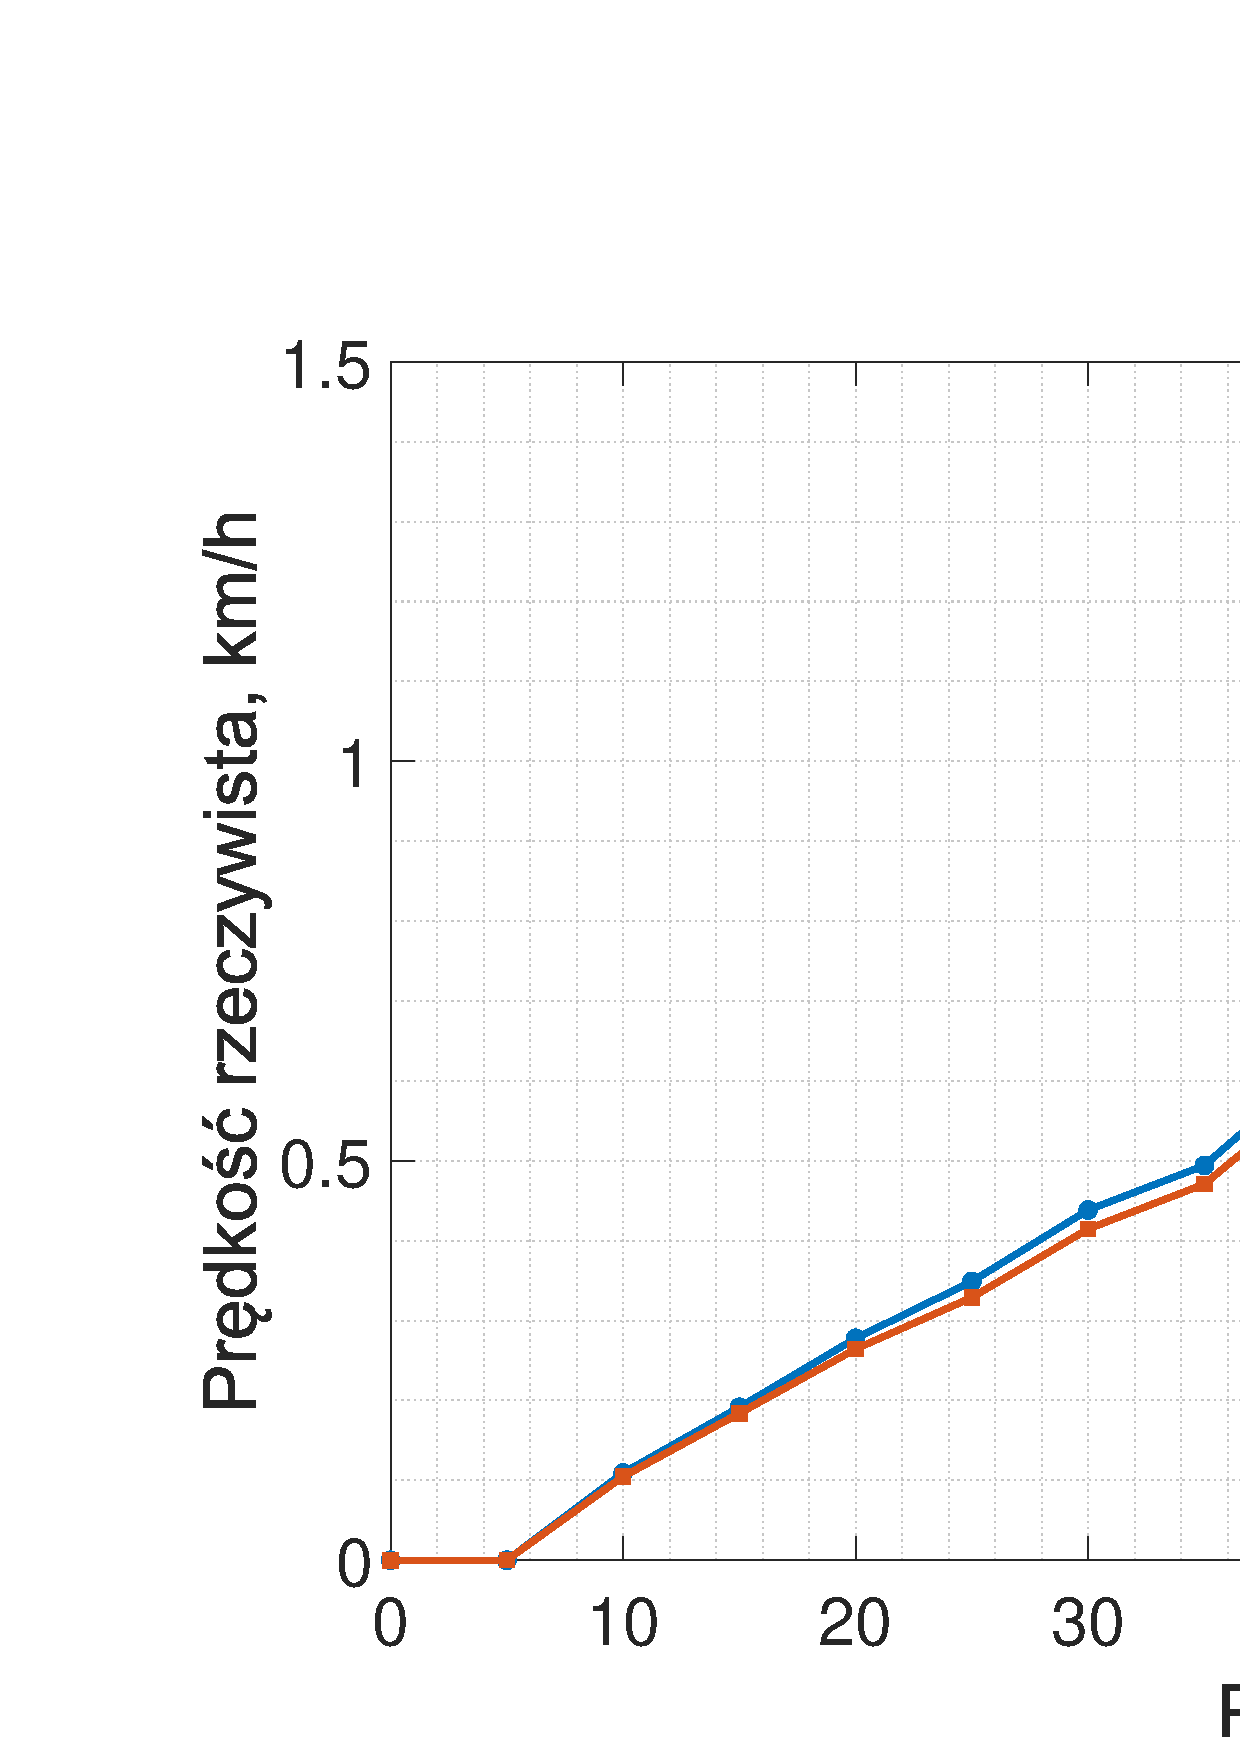
\includegraphics[scale=0.31]{images/charStat.png}
    \captionof{figure}{Charakterystyki statyczne silników}
    \label{fig:charstatjalowy}
\end{center}
\vspace*{-1cm}

\section{Strojenie regulatorów PID prowadzącego i śledzącego}
By ograniczyć ilość wykresów, których osobno byłoby kilkadziesiąt stron, kolejne iteracje zmiany tego samego parametru umieszczono na wspólnych wykresach. Strojenie odbywa się metodą doświadczalną.
\vspace*{-0.5cm}

\subsection*{Wzmocnienia proporcjonalne regulatora prowadzącego i~śledzącego}
Na Rysunku \ref{fig:strojeniekp} przedstawiono strojenie parametru K\textsubscript{P}.

\begin{center}
    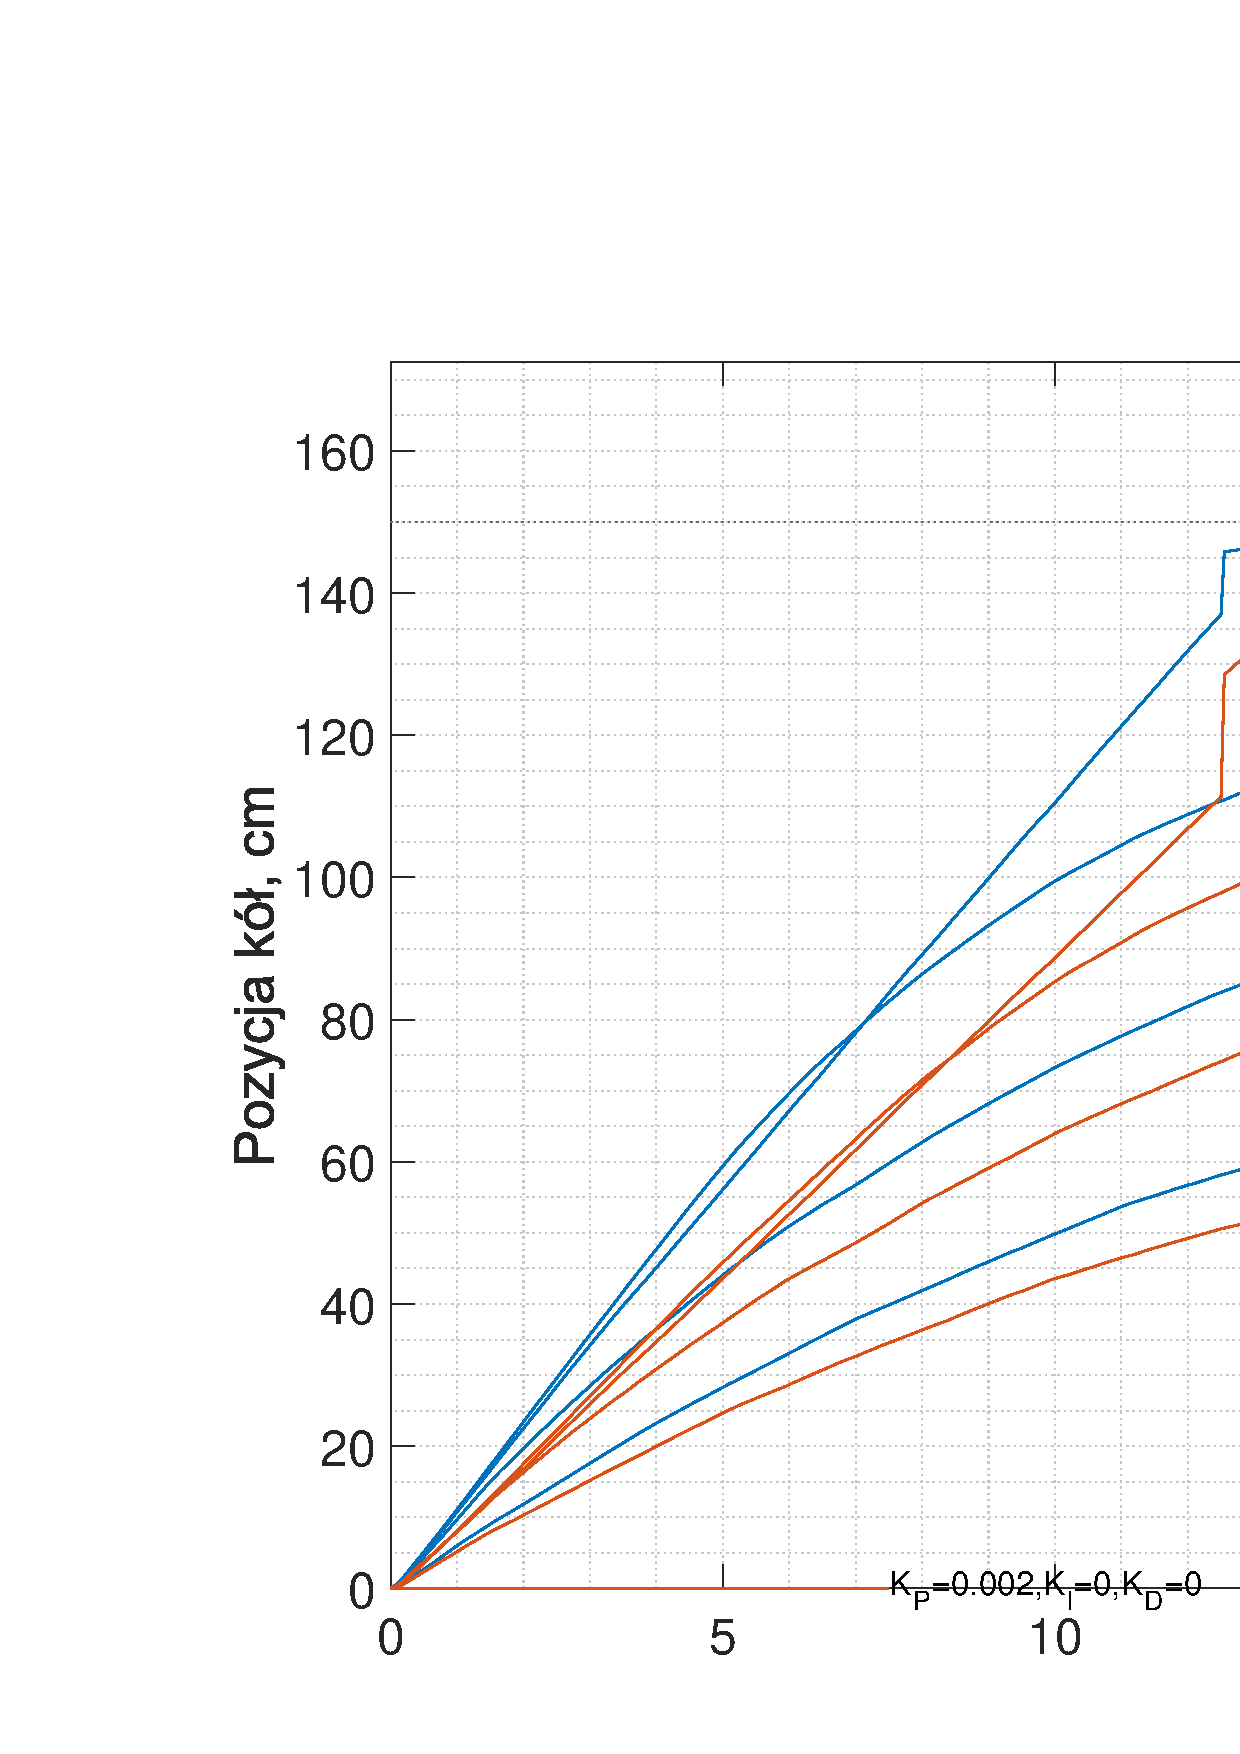
\includegraphics[scale=0.4]{images/strojenieKp.png}
    \captionof{figure}{Porównanie odpowiedzi układu na zmianę parametru K\textsubscript{P}}
    \label{fig:strojeniekp}
\end{center}

Widoczne jest, że wzmocnienie K\textsubscript{P}=0.002 jest zbyt małe, by pojazd ruszył z~miejsca (nie pokonuje oporu statycznego). Potrzebne jest wzmocnienie znajdujące się gdzieś w~przedziale K\textsubscript{P}$\in \left(0.002;0.006\right)$. Dla K\textsubscript{P}=0.1 uchyb jest bardzo mały, nawet bez części całkującej. Widoczny jest nagły skok odpowiedzi dla K\textsubscript{P}=0.1 pomiędzy 12~a~13~sekundą, którego powód jest nieznany. Jedną z~hipotez jest utracenie przez koła przyczepności na ułamek sekundy, tym samym wpadając w~lekki poślizg i~zwiększając obroty. Możliwy jest również inny błąd pomiaru.

\subsection*{Dodanie członu całkującego regulatora prowadzącego i śledzącego}
Na Rysunku \ref{fig:strojenieki} przedstawiono zmianę odpowiedzi układu po dodaniu parametru K\textsubscript{I} i~jednoczesnej modyfikacji K\textsubscript{P}.
\begin{center}
    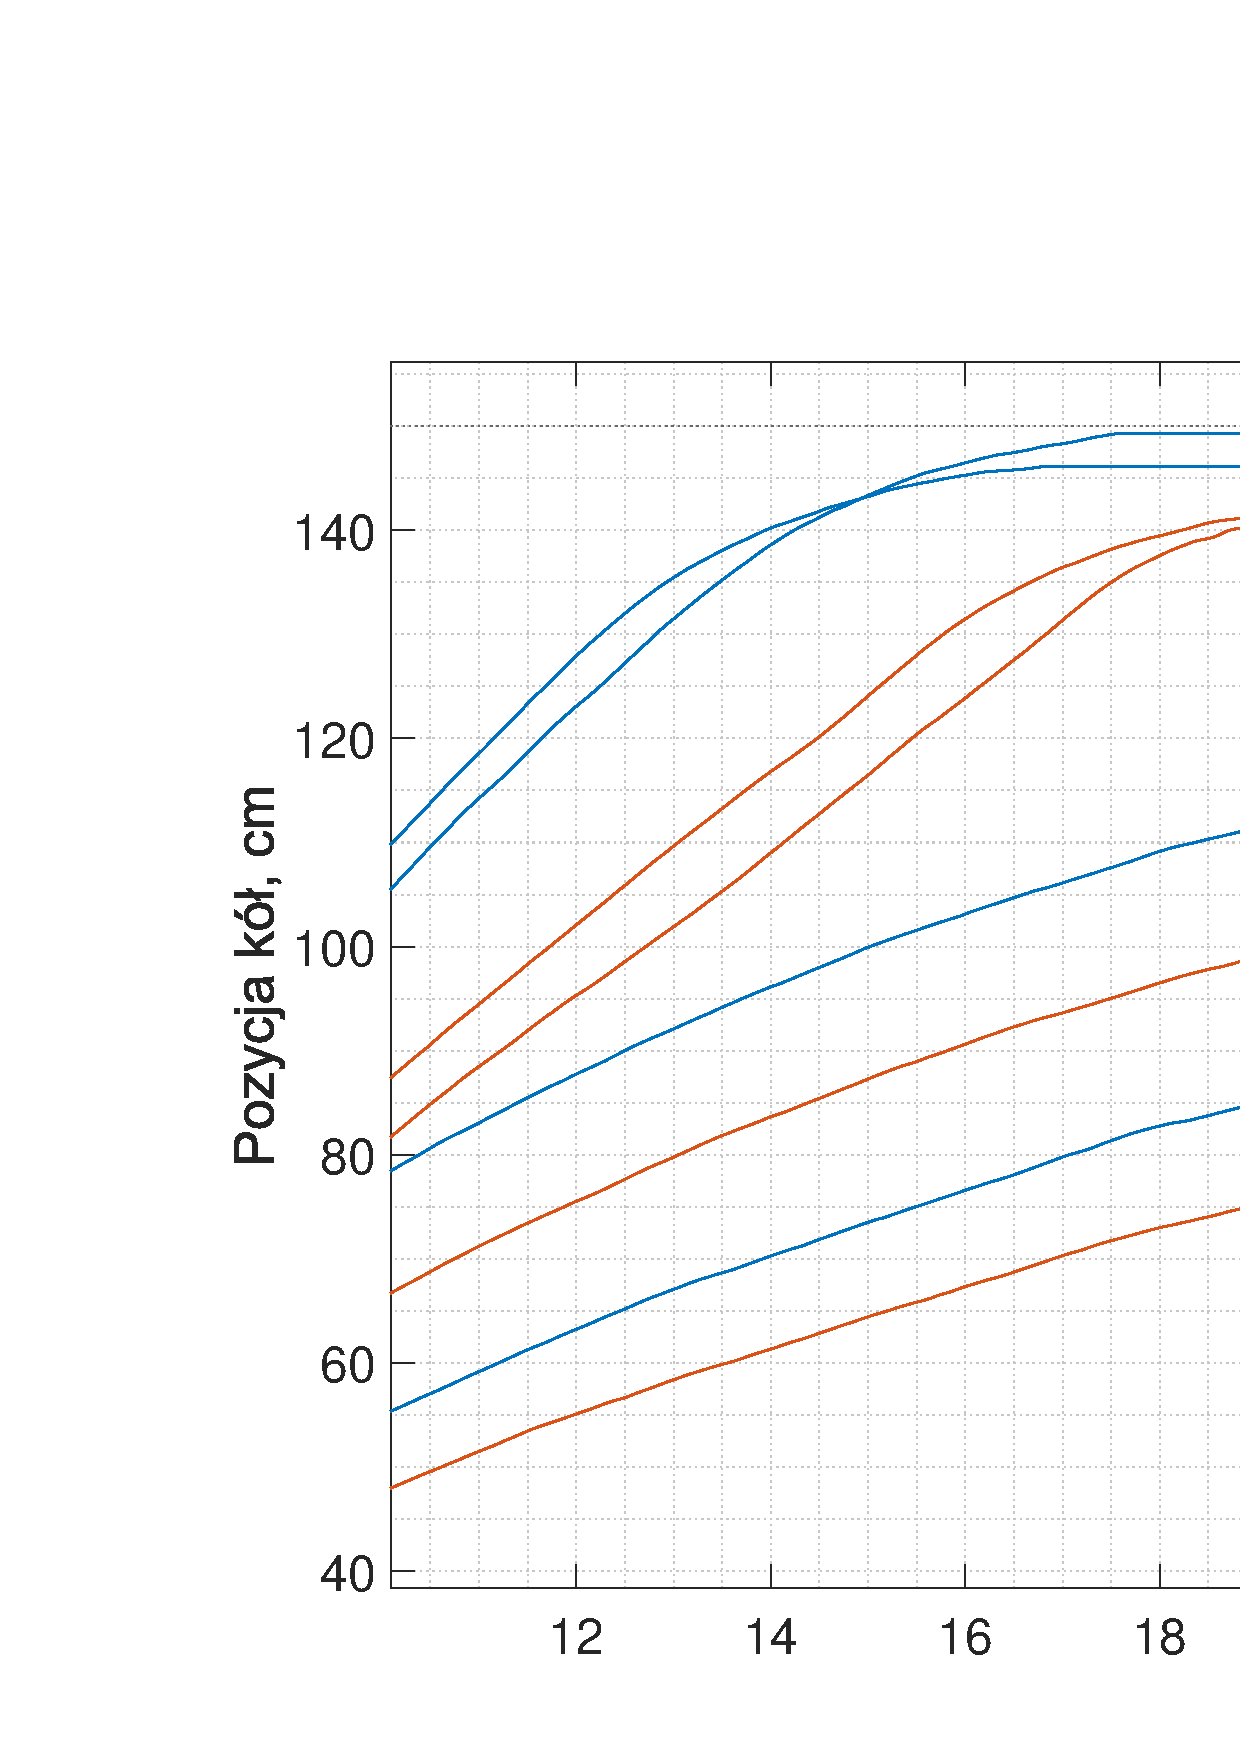
\includegraphics[scale=0.4]{images/strojenieKi.png}
    \captionof{figure}{Porównanie odpowiedzi układu na zmianę parametrów K\textsubscript{P} i K\textsubscript{I}}
    \label{fig:strojenieki}
\end{center}

Jak widać, nawet dla K\textsubscript{P}=0.05 czyli mniejszego niż najlepsze uzyskane w~poprzednim kroku, używając wzmocnienia K\textsubscript{I}=1, uchyb koła prowadzącego zostaje zniwelowany do wartości bliskiej 0. Jako że koło śledzące jest tym, które w~następnym kroku zostanie zsynchronizowane z~prowadzącym, a~samo koło prowadzące daje dobrą odpowiedź na aktualne parametry nie oscylując przy tym, wzmocnienie K\textsubscript{D} pozostanie wyzerowane, tym samym nie dodając do sygnału części różniczkującej regulatora.~W dalszych krokach używane będą parametry regulatorów K\textsubscript{P}=0.05, K\textsubscript{I}=1, oraz K\textsubscript{D}=0.

\section{Strojenie regulatora PID synchronizującego}
\subsection{Wzmocnienie różniczkujące}
Kolejnym krokiem jest dodanie regulatora PID synchronizującego koło śledzące z docelowym, zaczynając od części proporcjonalnej. Wykresy są zbyt blisko siebie by móc wyciągnąć wnioski, dlatego umieszczono dodatkowe przybliżenie. Różnice między poszczególnymi odpowiedziami w stanie ustalonym sprowadzają się do różnic w fizycznym wykonaniu przejazdu przez pojazd, czego należy się spodziewać. Strojenie wzmocnienia proporcjonalnego posiada mały wpływ na zbliżanie się do siebie odpowiedzi kół w części wykresu odpowiedzialnej za stan nieustalony. Odpowiedzi układu widoczne na Rysunku \ref{fig:strojenieskp}.

\begin{center}
    \includegraphics[scale=0.37]{images/strojenieSP.png}
    \captionof{figure}{Porównanie odpowiedzi układu na zmianę parametru K\textsubscript{P} regulatora synchronizującego}
    \label{fig:strojenieskp}
\end{center}

\subsection*{Dodanie składowej całkującej}
Po dodaniu członu całkującego do regulatora synchronizującego, zaczęły się widocznie wyłaniać pary kół z poszczególnych pomiarów. Wzmocnienie członu całkującego z powodzeniem zmniejszyło więc uchyb pomiędzy kołem prowadzącym a śledzącym, niestety nie do 0. Z wykresu ciężko odczytać konkretne pary i ich wartości, dlatego obliczenia przeprowadzono w MATLABie. Dla każdej próbki odjęto pozycję silnika śledzącego od prowadzącego. Następnie z otrzymanego wektora wyciągnięto średnią, a operację powtórzono dla wszystkich pomiarów (zmian K\textsubscript{I}), tym samym otrzymując wektor średnich błędów o długości równej ilości pomiarów. Najlepszym wynikiem charakteryzuje się K\textsubscript{I}=3, osiągając średni uchyb między pozycją kół na całym przebiegu na poziomie 0.12 cm. Przebiegi widoczne są na Rysunku \ref{fig:strojenieskpi}. Tak jak poprzednio, nie jest konieczne użycie członu różniczkującego.
\begin{center}
    \includegraphics[scale=0.37]{images/strojenieSPI.png}
    \captionof{figure}{Porównanie odpowiedzi układu na zmianę parametru K\textsubscript{I} regulatora synchronizującego}
    \label{fig:strojenieskpi}
\end{center}

Dla najlepszego wyniku, na Rysunku \ref{fig:finalneprzebiegi} przedstawiono prędkość kół, oraz w Tabeli \ref{tab:finalneparametrypid} końcowe parametry PID.

\begin{center}
    \includegraphics[scale=0.37]{images/wykresyfinalne.png}
    \captionof{figure}{Przedstawienie przebiegów pozycji silników oraz prędkości zadanej i rzeczywistej dla najlepszych parametrów PID}
    \label{fig:finalneprzebiegi}
\end{center}

\newpage

\begin{table}[!h]
\begin{tabular}{c|c|c|}
\cline{2-3}
\textbf{}                & Sygnały niezależne     & Sygnał zależny         \\ \hline
\multicolumn{1}{|c|}{K\textsubscript{P}} & 0.05                   & 0.2                    \\ \hline
\multicolumn{1}{|c|}{K\textsubscript{I}} & 1                      & 3                      \\ \hline
\multicolumn{1}{|c|}{K\textsubscript{D}} & \multicolumn{1}{c|}{0} & \multicolumn{1}{c|}{0} \\ \hline
\end{tabular}
\caption{Finalne parametry regulatorów PID dla najlepszego przebiegu}
\end{table}
\label{tab:finalneparametrypid}

Jak widać, dla finalnych parametrów uchyb od wartości zadanej jest bardzo mały, odczytany z wykresu wynosi 1.11 cm dla lewego koła i 1.46 cm dla prawego. Uchyb między kołami w stanie ustalonym wynosi --0.35 cm. Wyniki są więc bardzo dokładne biorąc pod uwagę warunki doświadczenia. Wadą są oscylacje prędkości zadanej lewego silnika spowodowane wysokim wzmocnieniem całkującym, które na szczęście w dużo mniejszym stopniu przekładają się na oscylacje realnej prędkości, oraz są zupełnie niewidoczne na przebiegu pozycji.